\documentclass[UTF8]{mcmthesis}
    % \usepackage{ctex}           % 暂时需要中文时添加, 最后注释掉即可
    \mcmsetup {
        tcn = 114514, problem = ABCDEF,    %% tcn is team control number
        titleinsummary = true,             %% title appears on summary sheet
    }

    % 调整 \item 的间距 
    \usepackage{paralist}
        \let\itemize\compactitem
        \let\enditemize\endcompactitem
        \let\enumerate\compactenum
        \let\endenumerate\endcompactenum
        \let\description\compactdesc
        \let\enddescriprion\endcompactdesc
    % 调整公式和正文的间距 (公式和正文更紧凑)
    \makeatletter
    \renewcommand\normalsize {
        % \@setfontsize\normalsize\@xpt\@xiipt
        \abovedisplayskip 5\p@ \@plus2\p@ \@minus5\p@
        \abovedisplayshortskip \z@ \@plus3\p@
        \belowdisplayshortskip 5\p@ \@plus3\p@ \@minus3\p@
        \belowdisplayskip \abovedisplayskip
        \let\@listi\@listI
    }
    \makeatother

    % \renewcommand{\baselinestretch}{1.2}      % 行间距
    \setlength{\parskip}{0.5em}                 % 段间距

    % 以下三种字体都太丑, 不建议使用()
    % \usepackage{mathptmx}     %% 数学公式罗马字体,对公式和正文都起作用
    % \usepackage{txfonts}      %% 数学公式罗马字体,对公式和正文都起作用
    % \usepackage{mathpazo}     %% COMAP 官方版物字体,对公式和正文都起作用
    % 一些重命名 ↓
    % \providecommand{\diff}{\mathop{}\!\mathrm{d}} %% 微分符号,正体 d
    % \providecommand{\me}{\mathrm{e}}              %% 无理数,正体 e
    % \providecommand{\mi}{\mathrm{i}}              %% 虚数单位,正体 i

    %% 设置目录节标题后加点
    \usepackage[titles]{tocloft}
    \renewcommand\cftsecdotsep{\cftdotsep}
    \renewcommand{\appendixpagename}{\Large\bfseries Appendices}

    %% 定制 Synopsis 页目录
    %% 根据需要把 Synopsis 改为 Memo or Handout 等等
    \fancypagestyle{Synopsis} {
        \fancyhf{}
        \lhead{\sffamily \team}
        \rhead{\sffamily Synopsis}
    }
    \title{\bfseries Title}  % 题目
  
\begin{document}
    \begin{summary}
        Lorem, ipsum dolor sit amet consectetur adipisicing elit. Minima vitae doloremque maxime similique, reiciendis blanditiis in dolore dolores necessitatibus, deserunt, quibusdam sapiente delectus nulla? Distinctio, eaque non. Accusantium, amet voluptate.

        \vspace{2em}
        \noindent\textbf{Key Words: } KeyWord1; KeyWord2
    \end{summary}

    \maketitle
    \newpage
    \tableofcontents

    \newpage
    \setcounter{page}{1}
    \section{Introduction}
        \subsection{Problem Background}
            \hspace*{2em}Lorem, ipsum dolor sit amet consectetur adipisicing elit. Minima vitae doloremque maxime similique, reiciendis blanditiis in dolore dolores necessitatibus, deserunt, quibusdam sapiente delectus nulla? Distinctio, eaque non. Accusantium, amet voluptate. \cite{link}
            \[
                \int_{1926}^{+\infty} \text{Ha}(t)\mathrm{d}t
            \]
            Lorem, ipsum dolor sit amet consectetur adipisicing elit. Minima vitae doloremque maxime similique, reiciendis blanditiis in dolore dolores necessitatibus, deserunt, quibusdam sapiente delectus nulla? Distinctio, eaque non. Accusantium, amet voluptate. 
            \begin{figure}[htpb]
                \centering
                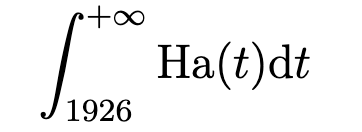
\includegraphics[width = .4\textwidth]{test}
                \vspace{-1em}
                \caption{Ha}
                \label{fig:1}
            \end{figure}
            
            Figure \ref{fig:1}.Lorem, ipsum dolor sit amet consectetur adipisicing elit. Minima vitae doloremque maxime similique, reiciendis blanditiis in dolore dolores necessitatibus, deserunt, quibusdam sapiente delectus nulla? Distinctio, eaque non. Accusantium, amet voluptate. 


        \subsection{Restatement of the Problem}
            \begin{enumerate}
                \item 
            \end{enumerate}
        \subsection{Our work}
            \begin{enumerate}
                \item 
            \end{enumerate}
            

    \section{Assumptions}
        \begin{enumerate}
            \item 
        \end{enumerate}
        

    \section{Notation}
        \hspace*{2em}Important notations used in this paper are listed in the table below.
        \vspace{-.5em}
        \begin{table}[htbp]
            \centering
            \caption{Notations}
            \vspace{0.5em}
            \begin{tabular}{cc}
                \toprule                % 顶部线
                    \textbf{Symbols} & \textbf{Description} \\ 
                \midrule                % 中部线
                    $t$ & Time \\
                \bottomrule             % 底部线
            \end{tabular}
        \end{table}


    \section{Problem 1}
    \section{Problem 2}
    \section{Problem 3}
    \section{Results}
    \section{Model Evaluation}
        \subsection{Strengths}
            \begin{enumerate}
                \item 
            \end{enumerate}
            
        \subsection{Weaknesses}
            \begin{enumerate}
                \item 
            \end{enumerate}


    %\label{LastPage2}
    \addcontentsline{toc}{section}{References}
        \begin{thebibliography}{99}
            \bibitem{link}
            Steven J. Leon.
            Linear Algebra with Applications.
            China Machine Press, 51 (2019).
        \end{thebibliography}


    \begin{appendices}
        Here are simulation programmes we used in our model as follow.
        
        \vspace{.5em}
        \noindent(1)\quad \verb|hello.cpp|
        \vspace{.5em}
        \begin{lstlisting}[language = c++, numbers = left]
    #include <iostream>
    int main() {
        std::cout << "Hello, world!\n";
        return 0;
    }
        \end{lstlisting}

    \end{appendices}
\end{document}
